\scanpage{49}
\mspage{24}
For the necessity of b), we are immediately reduced to the case where $\unsure{V|U}$ is reduced to a point, where this reduces to the \deleted{``\unsure{conjectural consequence}'' of the preliminary \unsure{conjecture-question}.}

\margin{\figure{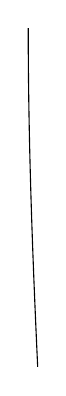
\begin{tikzpicture}\draw[thin] (0,0) .. controls (0,-1.5) and (0.06,-3) .. (0.12,-4.3);\end{tikzpicture}}}
\uline{Conjectural consequence} Let $\Gamma'\subset\operatorname{Im}(\mathcal E_U\longrightarrow\Gamma_{\mathbb{Q}}\unsure{)}$ be an open subgroup, corresponding to a field $k$ finite over $\mathbb{Q}$, let us consider a $k$-point of $U$, whence a lift $\Gamma'\unsure{-|\longrightarrow}\mathcal E_U$, so that $\Gamma'$ acts on $\unsure{\Pi|\pi}_{\unsure{U|K}}$. This being so\unsure{,} we have
\[
\unsure{\Pi|\pi}_U^{\Gamma'^\circ}=\{1\}.
\]

We shall subsequently study the relations between this \unsure{``}conjectural \inserted{consequence}'', and the preceding one (opposite in appearance!) concerning the $\mathcal E_K$.

The fundamental conjecture, on models implies the fundamental conjecture on fields, provided one takes care, in the latter, to restrict oneself to homomorphisms compatible with the model filtrations,
\margin{and it is better to restrict oneself to the \unsure{équivt.|equivalence} of a) and b) -- \unsure{the|the} \unsure{condition|conditions} c) on the centralizers \unsure{risk|risks} passing badly to $\varprojlim$}

More generally, taking \inserted{for $U$ \unsure{complete|complete|compact}} schemes, \deleted{\unsure{of dimension}} which are $\varprojlim$ of \unsure{anabelian|anabelian} \deleted{\unsure{schemes}} \inserted{elementary models}, with transition morphisms affine \inserted{open immersions}
\margin{48}
